In this section we summarize the tests on fit behavior using data. 
First, we invetigate fit behaviors in the control regions. 
Second, the change in nuiscance parameters by nominal fit is examined.  

%%%%%%%%%%%%%%%%%%%%%%%%%%%%%%%%%%%%%%%%%%%
\subsection{Control region}
There are following control regions where we can do the tests.

\begin{itemize}
    \item{\textbf{Same-sign \M\M~events} \\}  
        The sign requirement on the leptons is flipped. To get more statistics, 
        events in $|\mll - \mZ| < 15 \GeV$ are includeid. Instead of DYMVA, $minMET>35\GeV$
        is applied because requiring same sign reduces DY contribution (i.e. charge flip rate
        of muons is very small). This contral region is dominated by W+jets(\M), \Wgstar, and WZ/ZZ.
    \item{\textbf{Top-enriched sample} \\} 
        The top-veto requirement is flipped. This control region is dominated by top, WW, and Wjets.
%    \item{\textbf{WW-enriched} : }
%        $\mll > 70~\GeV$ is applied. This control region is dominated by WW, top, and Wjets.
%    \item Tri-lepton : ...  
\end{itemize}

The rest of selections are identical to the 2D analysis at $\mHi=125\GeV$.
In each test we perform a Maximum Likelihood fit with signal strength floated 
and check how normalizations of signal and background change.
Since signal contains only opposite sign di-lepton pairs, we use these events as signal 
in the test on same sign \M\M~events. The full 8 TeV data($\mathcal{L}=\intlumiEightTeV$) is used for the study.

Here is the summary of tests. Details(tables and plots) can be found in the appendix \ref{sec:appendix_fitvalidataion}. 
\begin{itemize}
    \item{\textbf{Same-sign \M\M~events} (Table \ref{tab:fitval_norm_ssmm_0j}-\ref{tab:fitval_norm_ssmm_1j}) \\ }  
        Signal contribution is close to 0 after fit. This means fit is able to 
        get the correct normalization when signal does not exist. Of the background 
        processes, WZ/ZZ and \Wgstar are not shifted, but Wjets($\mu$) is decreased by 30-40\% by fit.   
        This indicates a possible over-esitmation of Wjets($\mu$) background.  
    \item{\textbf{Top-enriched sample} (Table \ref{tab:fitval_norm_top_0j}-\ref{tab:fitval_norm_top_1j}) \\ } 
        In 0jet bin signal changed by -200\%, but the size of signal with respect to the total background 
        is only 1 \%. Therefore, change in the signal component is not significant. 
        Shift in backgrounds is not significant except for top in the 1jet bin. 
        Given that 94\% of the total background is from top, fit adjusts top to match data.  
%    \item{\textbf{WW-enriche}(Table \ref{tab:fitval_norm_ww_0j}-\ref{tab:fitval_norm_ww_1j}) : } 
%    \item Tri-lepton : ...  
\end{itemize} 

The conclusion is that fit does not show any anomalous behavior
when it is performed on the two control samples. Fit is able to assign 
proper normalizations of processes based on data.   


%%% SS mm 0jet
\begin{table}[ht!]
\begin{center}
\begin{tabular}{c|cc|cc}
\hline
\hline
Process &    N(prefit) &   N(postfit) & Difference(yield) &  Difference(\%)  \\  
\hline
\hline
ZH          &        0.0 &        0.0 &        0.0 &        0.0        \\
WH          &        3.4 &       -0.1 &       -3.6 &     -104.4        \\
qqH         &        1.5 &       -0.1 &       -1.6 &     -104.4        \\
ggH         &      129.2 &       -5.6 &     -134.8 &     -104.4        \\
\hline
qqWW        &        0.1 &        0.0 &        0.0 &        0.0        \\
ggWW        &        0.0 &        0.0 &        0.0 &        0.0        \\
\hline
WZ/ZZ       &       54.1 &       58.4 &        4.3 &        7.9        \\
\hline
Top         &        0.9 &        0.0 &        0.0 &        0.0        \\
\hline
Zjets       &        0.0 &        0.0 &        0.0 &        0.0        \\
\hline
Wjets($e$)  &        0.0 &        0.0 &        0.0 &        0.0        \\
Wjets($\mu$)&      122.7 &       88.8 &      -33.8 &      -27.6        \\
\hline
W$\gamma$   &        0.0 &        0.0 &        0.0 &        0.0        \\
W$\gamma$*  &       57.0 &       62.7 &        5.7 &       10.0        \\
\hline
Ztt         &        0.0 &        0.0 &        0.0 &        0.0        \\
\hline
\hline
\end{tabular}
\caption{Pre- and post-fit normalizations in same sign \M\M~events in 0jet bin. }
\label{tab:fitval_norm_ssmm_0j}
\end{center}
\end{table}

%%% SS mm 1jet
\begin{table}[ht!]
\begin{center}
\begin{tabular}{c|cc|cc}
\hline
\hline
Process     &    N(prefit) &   N(postfit) & Difference(yield) &  Difference(\%)  \\  
\hline
\hline
ZH          &        0.0 &        0.0 &        0.0 &        0.0        \\
WH          &        3.0 &        0.0 &       -3.0 &     -100.0        \\
qqH         &        5.4 &        0.0 &       -5.4 &     -100.0        \\
ggH         &       42.8 &        0.0 &      -42.8 &     -100.0        \\
\hline
qqWW        &        0.1 &        0.0 &        0.0 &        0.0        \\
ggWW        &        0.0 &        0.0 &        0.0 &        0.0        \\
\hline
WW/ZZ       &       26.1 &       30.3 &        4.2 &       16.2        \\
\hline
Top         &        3.5 &        4.3 &        0.8 &       23.5        \\
\hline
Zjets       &        0.0 &        0.0 &        0.0 &        0.0        \\
\hline
Wjets($e$)  &        0.0 &        0.0 &        0.0 &        0.0        \\
Wjets($\mu$)&       87.1 &       45.2 &      -41.9 &      -48.1        \\
\hline
W$\gamma$   &        0.0 &        0.0 &        0.0 &        0.0        \\
W$\gamma$*  &        6.8 &        7.6 &        0.8 &       11.5        \\
\hline
Ztt         &        0.0 &        0.0 &        0.0 &        0.0        \\
\hline
\hline
\end{tabular}
\caption{Pre- and post-fit normalizations in same sign \M\M~events in 1jet bin. }
\label{tab:fitval_norm_ssmm_1j}
\end{center}
\end{table}


%%% Top-enriched 0jet
\begin{table}[ht!]
\begin{center}
\begin{tabular}{c|cc|cc}
\hline
\hline
Process     &    N(prefit) &   N(postfit) & Difference(raw) &  Difference(\%)  \\  
\hline
\hline
ZH          &        0.0 &        0.0 &        0.0 &        0.0        \\
WH          &        0.8 &        0.0 &        0.0 &        0.0        \\
qqH         &        0.2 &        0.0 &        0.0 &        0.0        \\
ggH         &        8.1 &       -7.8 &      -15.8 &     -196.5        \\
\hline
qqWW        &      135.2 &      151.2 &       16.0 &       11.8        \\
ggWW        &        7.8 &        8.8 &        1.0 &       13.2        \\
\hline
WZ/ZZ       &       19.3 &       17.4 &       -1.9 &      -10.0        \\
\hline
Top         &      500.3 &      480.5 &      -19.8 &       -4.0        \\
\hline
Zjets       &        0.0 &        0.0 &        0.0 &        0.0        \\
\hline
Wjets($e$)  &       19.6 &       19.7 &        0.0 &        0.2        \\
Wjets($\mu$)&       54.8 &       64.2 &        9.4 &       17.1        \\
\hline
W$\gamma$   &        2.8 &        2.4 &       -0.4 &      -13.2        \\
W$\gamma$*  &       47.7 &       45.1 &       -2.6 &       -5.5        \\
\hline
Ztt         &        4.0 &        3.9 &       -0.0 &       -0.3        \\
\hline
\hline
\end{tabular}
\caption{Pre- and post-fit normalizations in the top-enriched region in 0jet bin.}
\label{tab:fitval_norm_top_0j}
\end{center}
\end{table}

%%% Top-enriched 1jet
\begin{table}[ht!]
\begin{center}
\begin{tabular}{c|cc|cc}
\hline
\hline
Process     &    N(prefit) &   N(postfit) & Difference(raw) &  Difference(\%)  \\  
\hline
\hline
ZH          &        0.0 &        0.0 &        0.0 &        0.0        \\
WH          &        1.1 &        1.0 &       -0.1 &       -7.9        \\
qqH         &        1.3 &        1.2 &       -0.1 &       -7.4        \\
ggH         &       10.9 &       10.0 &       -0.9 &       -8.3        \\
\hline
qqWW        &      156.0 &      166.7 &       10.7 &        6.9        \\
ggWW        &        6.0 &        6.0 &       -0.0 &       -0.3        \\
\hline
WZ/ZZ       &       33.2 &       33.2 &        0.0 &        0.1        \\
\hline
Top         &     5658.9 &     5423.9 &     -235.0 &       -4.2        \\
\hline
Zjets       &        0.0 &        0.0 &        0.0 &        0.0        \\
\hline
Wjets($e$)  &       39.2 &       32.8 &       -6.4 &      -16.3        \\
Wjets($\mu$)&      108.6 &      105.5 &       -3.1 &       -2.9        \\
\hline
W$\gamma$   &        6.1 &        6.2 &        0.0 &        0.5        \\
W$\gamma$*  &       10.7 &       10.9 &        0.2 &        1.7        \\
\hline
Ztt         &       20.2 &       19.2 &       -1.1 &       -5.3        \\
\hline
\hline
\end{tabular}
\caption{Pre- and post-fit normalizations in the top-enriched region in 1jet bin.}
\label{tab:fitval_norm_top_1j}
\end{center}
\end{table}


%%%%%%%%%%%%%%%%%%%%%%%%%%%%%%%%%%%%%%%%%%%
\subsection{Nuisances in the norminal fit}
In this section, we describe how nuiscance parameters change by the nominal fit. 
Fit is done on the full 8 TeV dataset in 0/1jet DF final states separately. 
Figure~\ref{fig:postnuisance} shows the pull of nuiscance parameters. The x-axis shows 
index of nuisance paramters. Gray region corresponds to input uncertainty($1\sigma$) of  
of each nuiscance. Solid line indicates the post fit value(central) and uncertainty(error bar)
of each nuisance. The outlier at index 18 in the 0jet is normalization nuiscance for 
$\wjetsm$.

%%%%%
\begin{figure}[!hbtp]
\centering
\subfigure[]{
\centering
\label{subfig:postnuisance_0j}
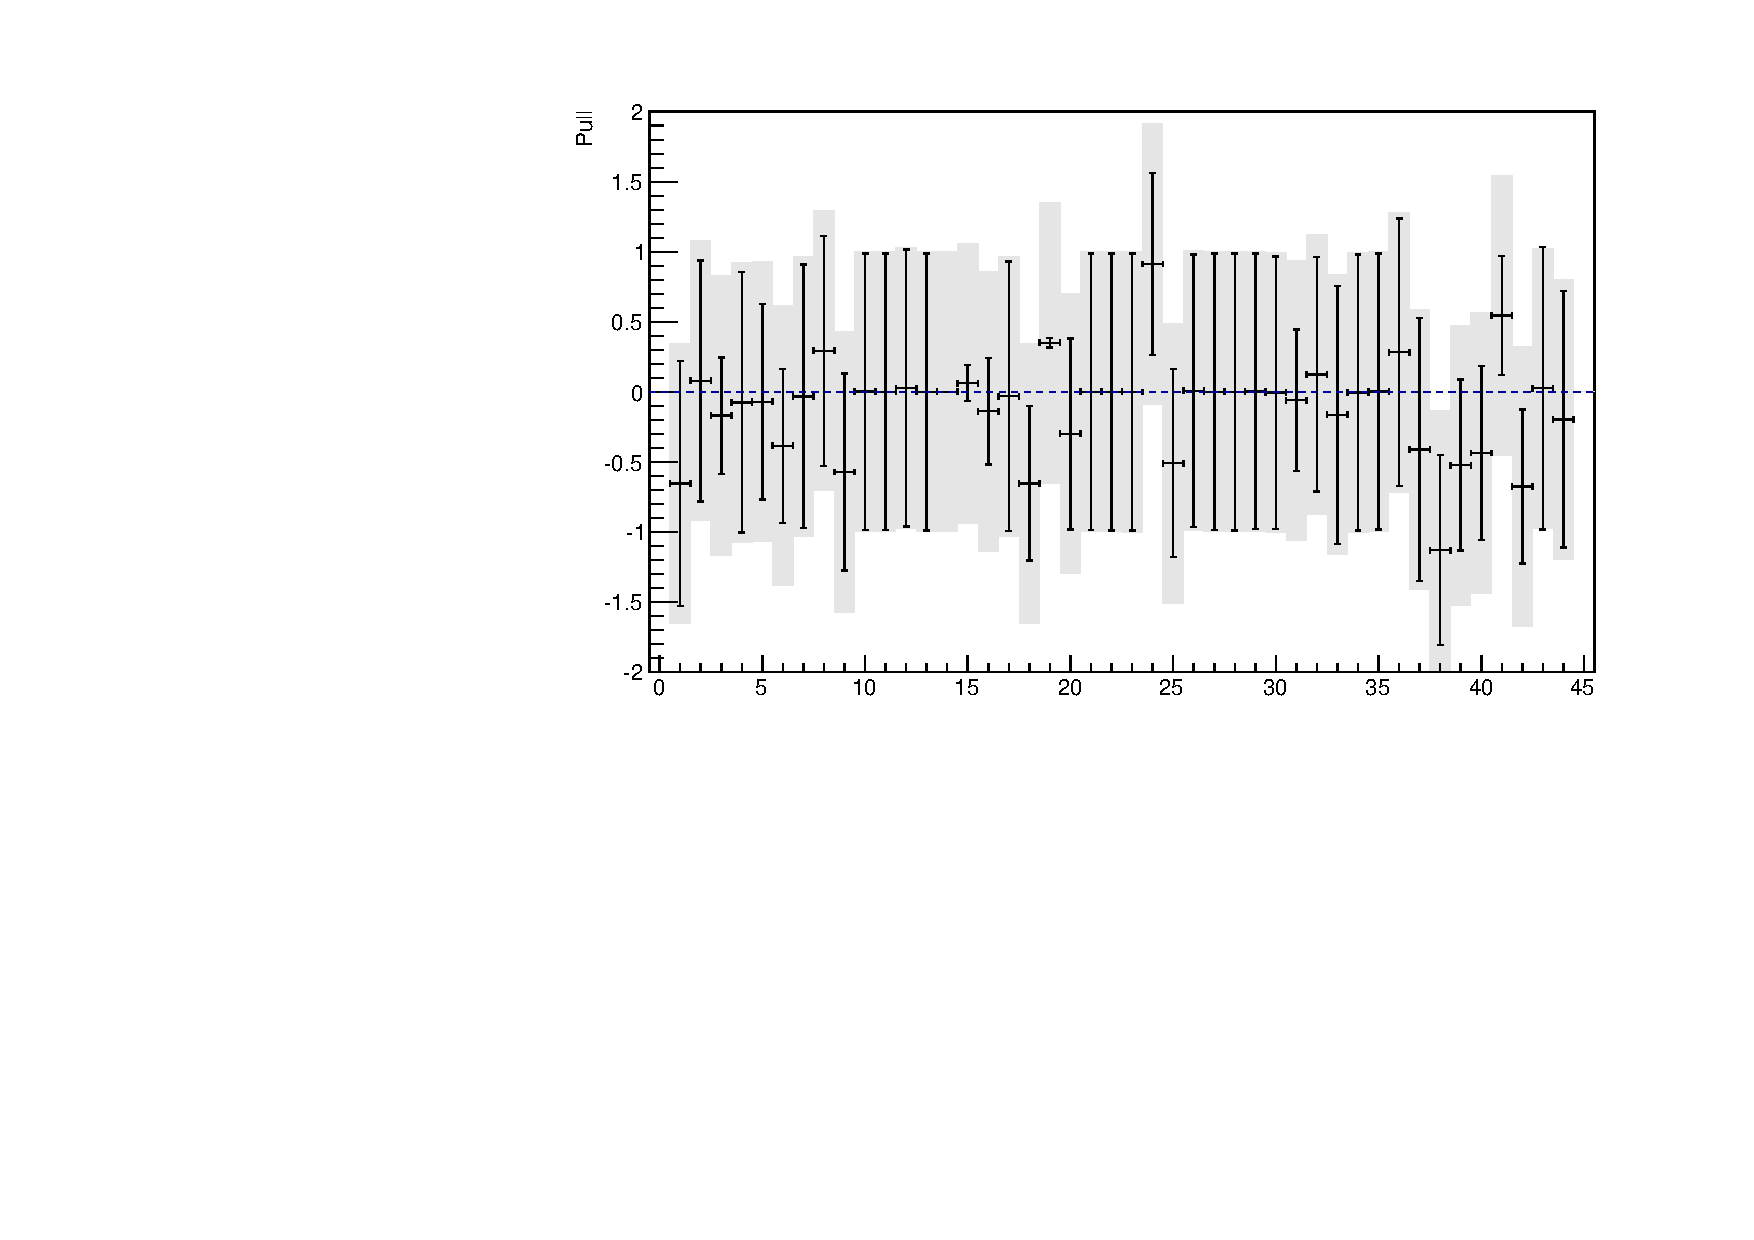
\includegraphics[width=.8\textwidth]{figures/limits_0j_shape_of_125-fit-125-all_Postnuisance.pdf}
}
\subfigure[]{
\centering
\label{subfig:postnuisance_1j}
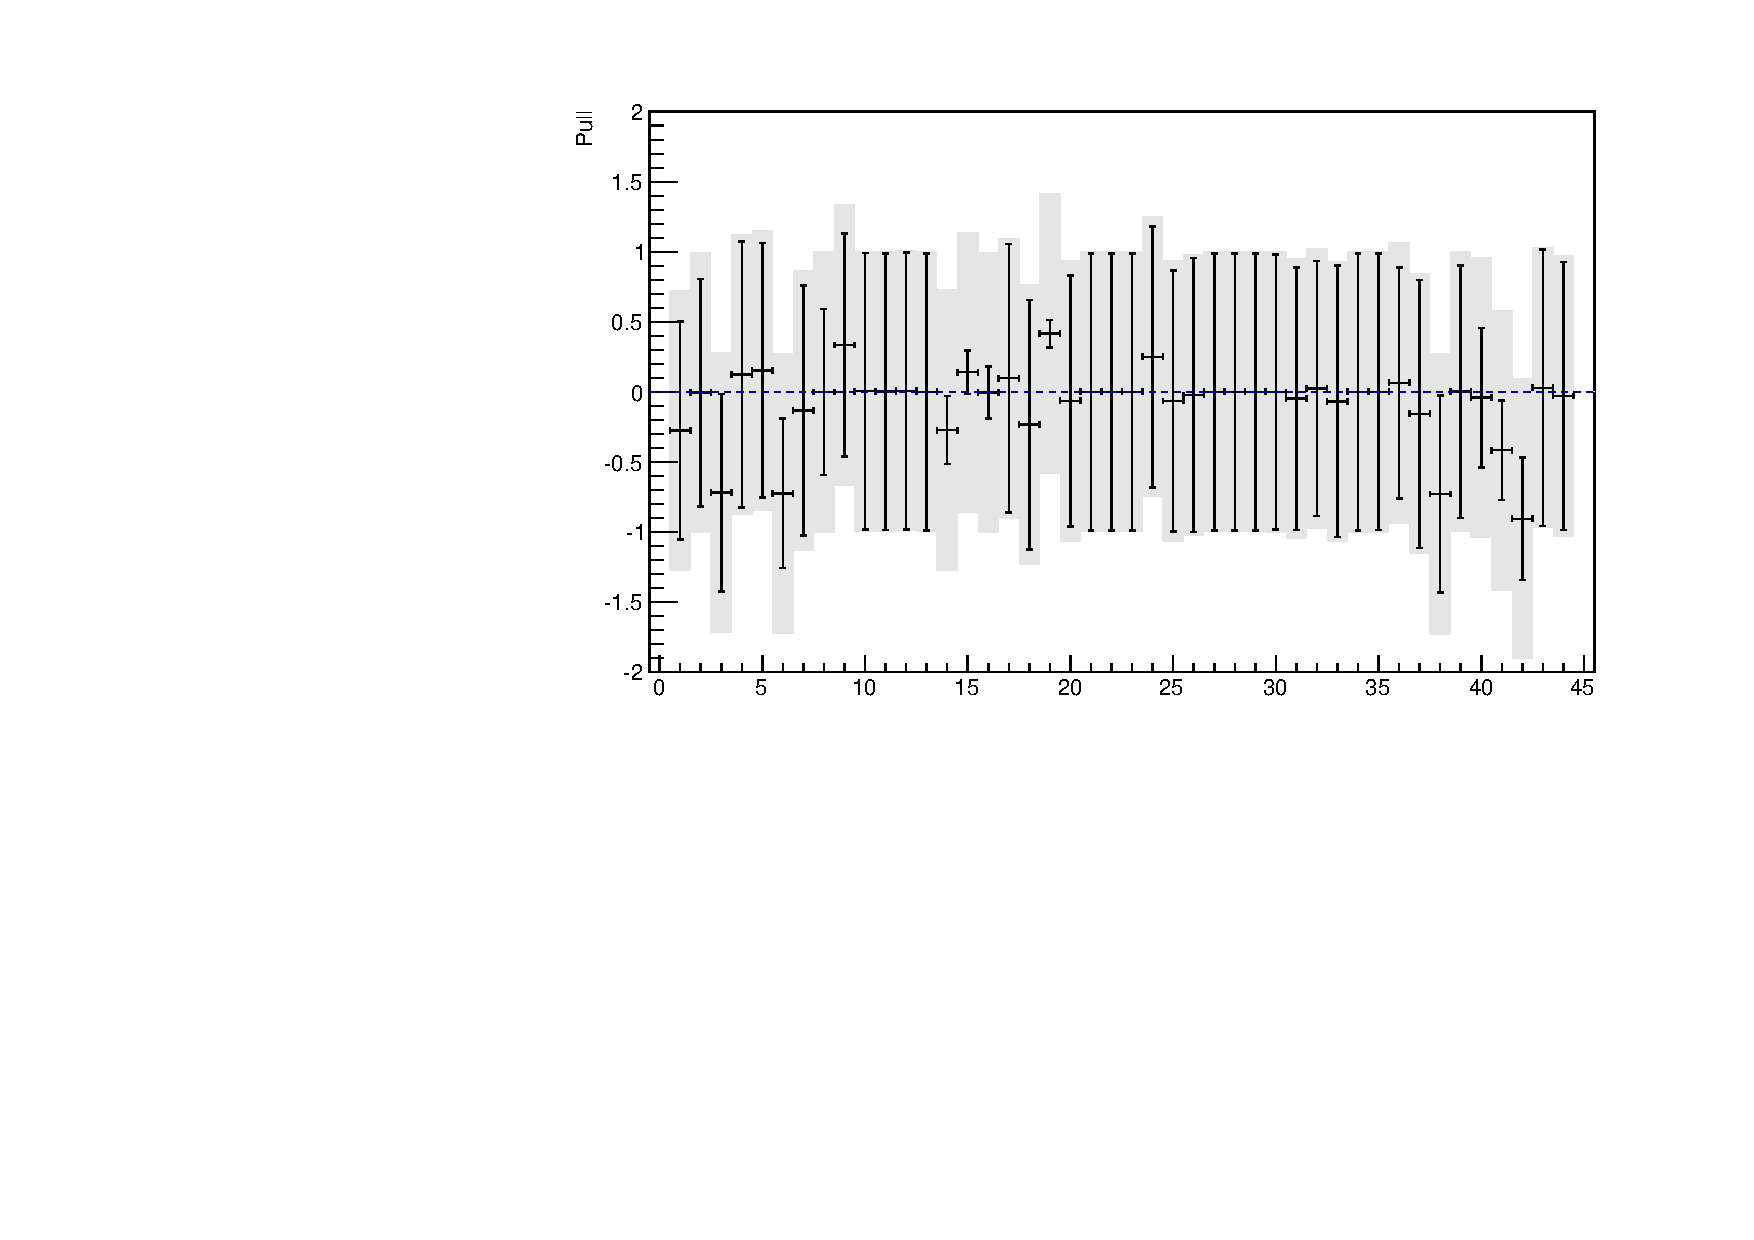
\includegraphics[width=.8\textwidth]{figures/limits_1j_shape_of_125-fit-125-all_Postnuisance.pdf}
}\\
\caption{Top(bottom) figure shows pull of nuisance paramters in 0(1)jet bin.
Gray region corresponds to input uncertainty($1\sigma$) of each nuiscance. 
Solid line indicates the post-fit value(central point) and uncertainty(error bar)
of each nuisance.} 
\label{fig:postnuisance}
\end{figure}

%%%%%%%%%%%%%%%%%%%%%%%%%%%%%%%%%%%%%%%%%%%
\subsection{Impact of different WW shapes on the observed signal strength} 

In 2D analysis we rely on MC for WW shapes. We use Madgraph+Pythia6 as a central shape 
and MC@NLO+Herwig6 with/without QCD scale variations as alternate shapes to account for 
shape variation. Because it is hard to validate the WW shape against data, we perform 
nominal fit with different set of central and alternate shapes. If the changes in the 
signal strength($\mu$) is small by changing shapes, we are safe in accounting for shape uncertainties.
So, we define relative movement of signal strength with respect to the nominal one.   
The movement is defined as 
\begin{equation} 
|\Delta\mu| = \frac{|\mu_{nominal} - \mu_{variation}|}{|\mu_{nominal}|}  
\end{equation} 
where $\mu_{nominal}$ is from our choice for analysis and $\mu_{variation}$ is from 
different combination of samples. To remain blinded, we take absolute value of 
difference so that we are not aware of direction of changes. 
Table \ref{tab:fitval_mu} shows $\Delta\mu$ with two different choices of central 
and alternate shapes. Expected significance does not change. Maximum $\Delta\mu$ is 12\%.
Thus, we conclude that signal strength is not sensitive to the choice of WW MC.

%%% 
\begin{table}[ht!]
\begin{center}
\begin{tabular}{c|c|c|c}
\hline \hline
Central shape               & Madgraph          & Powheg            & MC\@NLO           \\  
\hline 
Different generator         & MC\@NLO           & MC\@NLO           & Madgraph          \\  
\hline
Scale variation             & MC\@NLO up/down   & MC\@NLO up/down   & MC\@NLO up/down   \\  
\hline \hline
Expected significance       & 3.5               & 3.5               & 3.6               \\  
$\Delta\mu$                 & 0                 & 3\%               & 12\%               \\  
\hline \hline
\end{tabular}
\caption{Shift in signal strength by different choice of central and alternate shapes.}
\label{tab:fitval_mu}
\end{center}
\end{table}


